\documentclass[aspectratio=169,10pt]{beamer}
\usetheme{metropolis}
\usepackage{booktabs}
\usepackage{graphicx}
\usepackage{amssymb}
\makeatletter\newcommand{\tabinput}[1]{\@@input #1 }\makeatother
\newcommand{\Bfit}{B_{\mathrm{fit}}}
\newcommand{\Bval}{B_{\mathrm{val}}}
\newcommand{\FinalMacro}{0.9134}
\newcommand{\FinalAcc}{98.21}
\newcommand{\ReproMLR}{0.8967}
\newcommand{\PaperMLR}{0.8949}
\newcommand{\CalT}{0.133}
\newcommand{\EceRaw}{0.0041}
\newcommand{\EceT}{0.0070}
\newcommand{\RejCov}{95.2}
\newcommand{\RejAcc}{99.72}
\newcommand{\RejMacro}{0.9861}
\newcommand{\SeedStd}{0.012}
\newcommand{\GainOverRepro}{+0.0168}

\graphicspath{{../paper/figures/}}

\title{Stacking Handcrafted and Convolutional Features\\for Wafer Map Classification, Revisited}
\subtitle{Reproduction, Meta-Training Pitfalls, and Improvements}
\author{Kartikeya Gupta}
\institute{Indian Institute of Information Technology Sri City}
\date{}

\begin{document}
\maketitle

\begin{frame}{The problem}
\begin{itemize}
\item A \alert{wafer map} records which dies on a wafer failed electrical tests.
\item Failures form \alert{patterns}; each points to a different fault in fabrication $\Rightarrow$ automatic classification supports yield analysis.
\item WM-811K: 172,946 labeled wafers, 85\% ``None'' $\Rightarrow$ we report \alert{macro-F1}.
\end{itemize}
\vspace{0.3em}
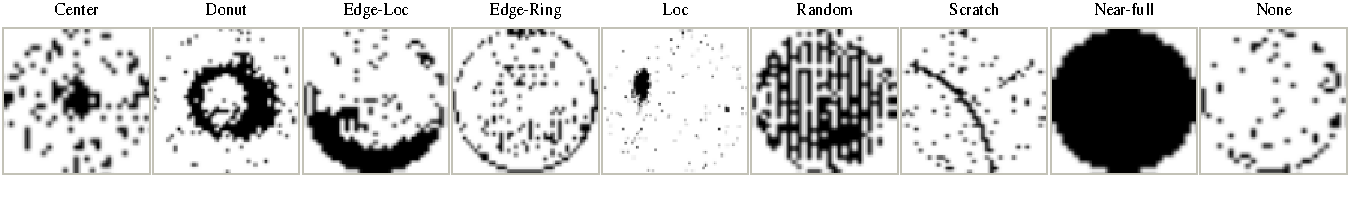
\includegraphics[width=\linewidth]{examples.pdf}\\
{\scriptsize One test wafer per class (dark = failed die).}
\end{frame}

\begin{frame}{The paper we reproduce}
Kang \& Kang, \emph{Computers in Industry} 129 (2021) 103450 (Elsevier)
\begin{enumerate}
\item \textbf{MFE+FNN}: 59 handcrafted features (region densities, Radon transform, defect geometry) $\to$ small neural network
\item \textbf{CNN}: VGG16, ImageNet-pretrained, on the $64\times64$ map
\item \textbf{Stacking-MLR}: ridge regression on both models' class probabilities $\to$ a per-class weight for each model
\end{enumerate}
\vspace{0.5em}
Reported: Stacking-MLR macro-F1 \alert{\PaperMLR}, better than either base model and four other baselines.
\end{frame}

\begin{frame}{Our contributions}
\begin{enumerate}
\item \textbf{Full reproduction} of all six models, at four training-set sizes
\item \textbf{A meta-training pitfall} in the public code, and its fix
\item \textbf{Controlled extensions}: test-time augmentation, XGBoost, CNN seed ensembles
\item \textbf{Selective prediction}: send uncertain wafers to an engineer
\end{enumerate}
\vspace{0.5em}
Rules: all choices on a validation split $B$; test set only for reporting; paired $t$-tests and wafer bootstrap intervals;
negative results reported.
\end{frame}

\begin{frame}{Protocol}
\begin{itemize}
\item Train 162,946 / test 10,000 (stratified)
\item Training set $\to$ $A$ (130,356): fit base models \quad $B$ (32,590): validation and meta-training
\item $B = \Bfit \cup \Bval$; base models early-stop on $\Bfit$
\item Selection score: two-fold cross-fit of the stacker over $B$
\item Inclusion rule: keep an extension if it beats the baseline by more than the run-to-run std
\end{itemize}
\end{frame}

\begin{frame}{Reproduction at full data}
\centering\footnotesize
\begin{tabular}{lccccl}
\toprule
& \multicolumn{2}{c}{macro-F1} & \multicolumn{2}{c}{micro-F1} & \\
\cmidrule(lr){2-3}\cmidrule(lr){4-5}
Model & ours & reported & ours & reported & runs \\
\midrule
\tabinput{../paper/tables/repro.tex}
\bottomrule
\end{tabular}\\[0.6em]
\normalsize All six models match or beat the paper. $^\dagger$Stacking-FNN fitted on $B$.
\end{frame}

\begin{frame}{The meta-training pitfall}
\begin{itemize}
\item Public code: stacker trained on the base models' predictions \alert{for their own training data}
\item There the models are almost always right and very confident $\Rightarrow$ the stacker learns ``always follow them''
\item Result: the rarest class (Near-full) is never predicted, macro-F1 0.6298 $\pm$ 0.0904
\item Class weights only hide it (0.8402 $\pm$ 0.0393, unstable)
\item \alert{Fix}: train the stacker on held-out data $B$ --- the classic advice for stacking
\item Linear MLR is far less affected than FNN or tree stackers
\end{itemize}
\end{frame}

\begin{frame}{Training-size sweep}
\begin{columns}[c]
\column{0.5\textwidth}
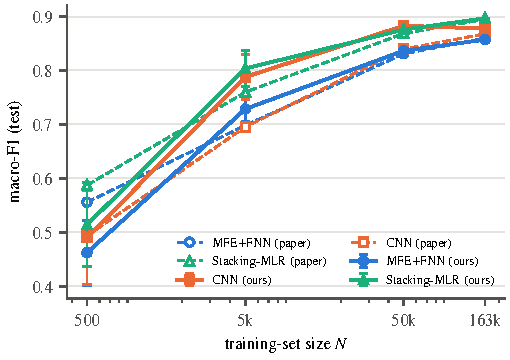
\includegraphics[width=\linewidth]{sweep.pdf}
\column{0.48\textwidth}
\begin{itemize}\small
\item $N \ge 5{,}000$: every model beats the paper
\item $N = 500$: noisy; rare classes often missing from 400 wafers
\item $N = 50{,}000$: MLR stack below our CNN under the paper's in-sample protocol --- the same pitfall
\end{itemize}
\end{columns}
\end{frame}

\begin{frame}{Extensions}
\centering\scriptsize
\begin{tabular}{lccc}
\toprule
Configuration & $B$ (MLR) & test (MLR) & test (FNN) \\
\midrule
\tabinput{../paper/tables/extensions.tex}
\bottomrule
\end{tabular}\\[0.6em]
\small TTA: average over 8 rotations/flips \quad CNN$\times$5: five CNN seeds averaged
\end{frame}

\begin{frame}{What helped, what did not}
\begin{columns}[T]
\column{0.48\textwidth}
\textbf{Helped}
\begin{itemize}\small
\item Test-time augmentation (significant on $B$)
\item XGBoost as the handcrafted-feature model
\item \alert{Five-CNN ensemble}: largest gain; seeds differ by $\pm$\SeedStd{} macro-F1 at equal loss
\end{itemize}
\column{0.48\textwidth}
\textbf{Did not help}
\begin{itemize}\small
\item A \emph{different} third model vs.\ a second seed
\item The paper's MFE+FNN once the CNN is an ensemble
\item Bagging XGBoost, class weights, mixed precision
\item Temperature scaling for MLR calibration
\end{itemize}
\end{columns}
\end{frame}

\begin{frame}{Final pipeline}
\begin{center}
\Large 5 CNNs (TTA) \;+\; XGBoost \;$\xrightarrow{\text{MLR}}$\; class
\end{center}
\vspace{0.5em}
\begin{itemize}
\item Test macro-F1 \alert{\FinalMacro} \quad (paper \PaperMLR, our reproduction \ReproMLR)
\item Accuracy \FinalAcc\%
\item Gain over reproduction \GainOverRepro{}, bootstrap interval excludes zero
\item Runnable from saved models: \texttt{predict.py}
\end{itemize}
\end{frame}

\begin{frame}{Selective prediction}
\begin{columns}[c]
\column{0.52\textwidth}
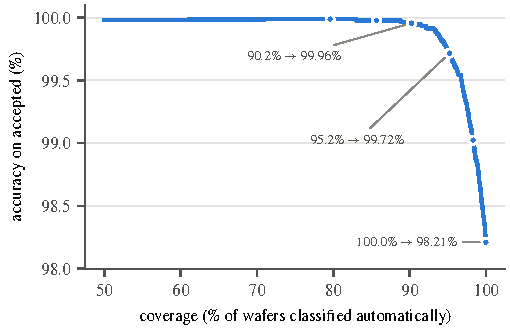
\includegraphics[width=\linewidth]{reject.pdf}
\column{0.46\textwidth}
\begin{itemize}\small
\item Confidence = max probability (temperature-scaled)
\item Thresholds chosen on $B$, applied to test
\item \alert{\RejCov\% automatic at \RejAcc\% accuracy}
\item Deferred: mostly Loc, Scratch, Edge-Loc; only 2\% of None
\end{itemize}
\end{columns}
\end{frame}

\begin{frame}{What the stack learns}
\begin{columns}[c]
\column{0.55\textwidth}
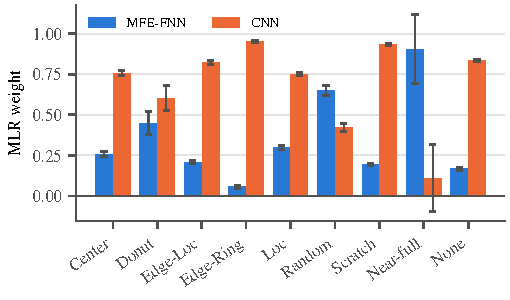
\includegraphics[width=\linewidth]{weights.pdf}
\column{0.43\textwidth}
\begin{itemize}\small
\item Handcrafted features carry \alert{Random} and \alert{Near-full} (global density)
\item CNN carries the spatial patterns (Edge-Ring, Scratch)
\item Matches the paper's Fig.~5
\item SHAP: eccentricity/solidity for Scratch, defect area for Near-full
\end{itemize}
\end{columns}
\end{frame}

\begin{frame}{Limitations}
\begin{itemize}
\item One fixed train/test split (paper: ten)
\item Near-full has 9 test wafers: one wafer $\approx$ 0.01 macro-F1
\item Test set consulted twice (always after selection on $B$)
\item Five replicates at $N=50{,}000$; MultiNN single run; preliminary model-selection tables not repeated
\end{itemize}
\end{frame}

\begin{frame}{Conclusion}
\begin{itemize}
\item The paper \alert{reproduces}: \ReproMLR{} vs \PaperMLR
\item Train the stacker on held-out outputs, never in-sample
\item The handcrafted branch helps a single CNN but not a CNN ensemble
\item Best: \alert{\FinalMacro} macro-F1; \RejCov\% of wafers at \RejAcc\% accuracy with a reject option
\end{itemize}
\vspace{1em}
\small Code: \url{github.com/Kartikeya2046/ML_wafer_detecting_using_stack_ensemble}
\end{frame}

\end{document}
